\chapter{Clustering Spectral Images}
\label{ch:spectra_image_clustering}

\begin{wrapfigure}{o}{0.63\textwidth}
    \vspace{-3.5cm}
    \centering
    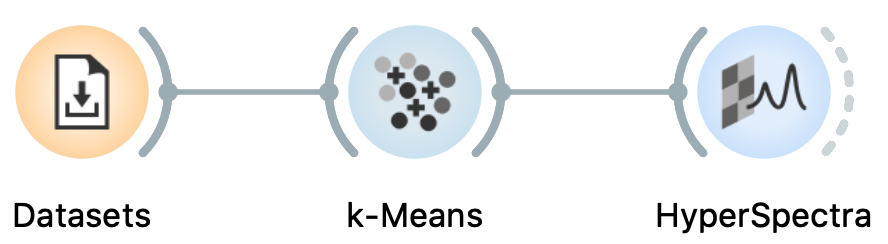
\includegraphics[scale=0.4]{graphics/ch-spectra_image_clustering/sp_image_clustering-fig1.png}
    \label{fig:spectra_image_clustering-fig1}
\end{wrapfigure}

We have already seen hierarchical clustering. Another clustering algorithm, k-Means, is much faster for data with lots of rows, like images, which contain a row (a spectrum) for each pixel. Still, for the liver-cirrhosis data, both approaches are fast. Here, we use \widget{k-Means} with k=3 clusters. 

\begin{figure*}[h]
  \vspace{-0.3cm}
  \newcommand{\kmeans}{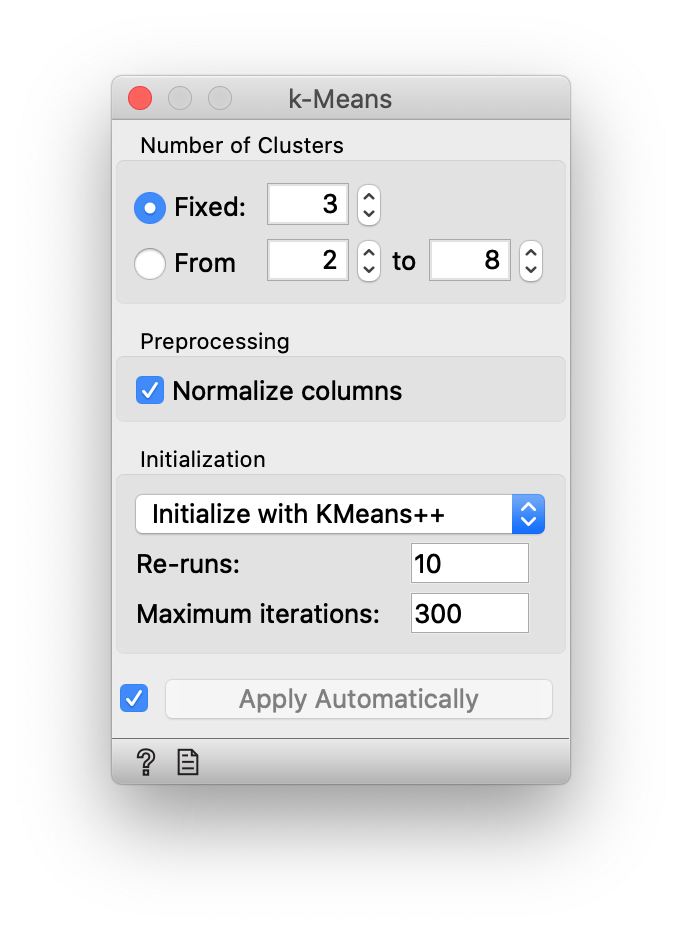
\includegraphics[scale=0.40]{graphics/ch-spectra_image_clustering/sp_image_clustering-fig2a.png}}
  \newcommand{\hyperspectra}{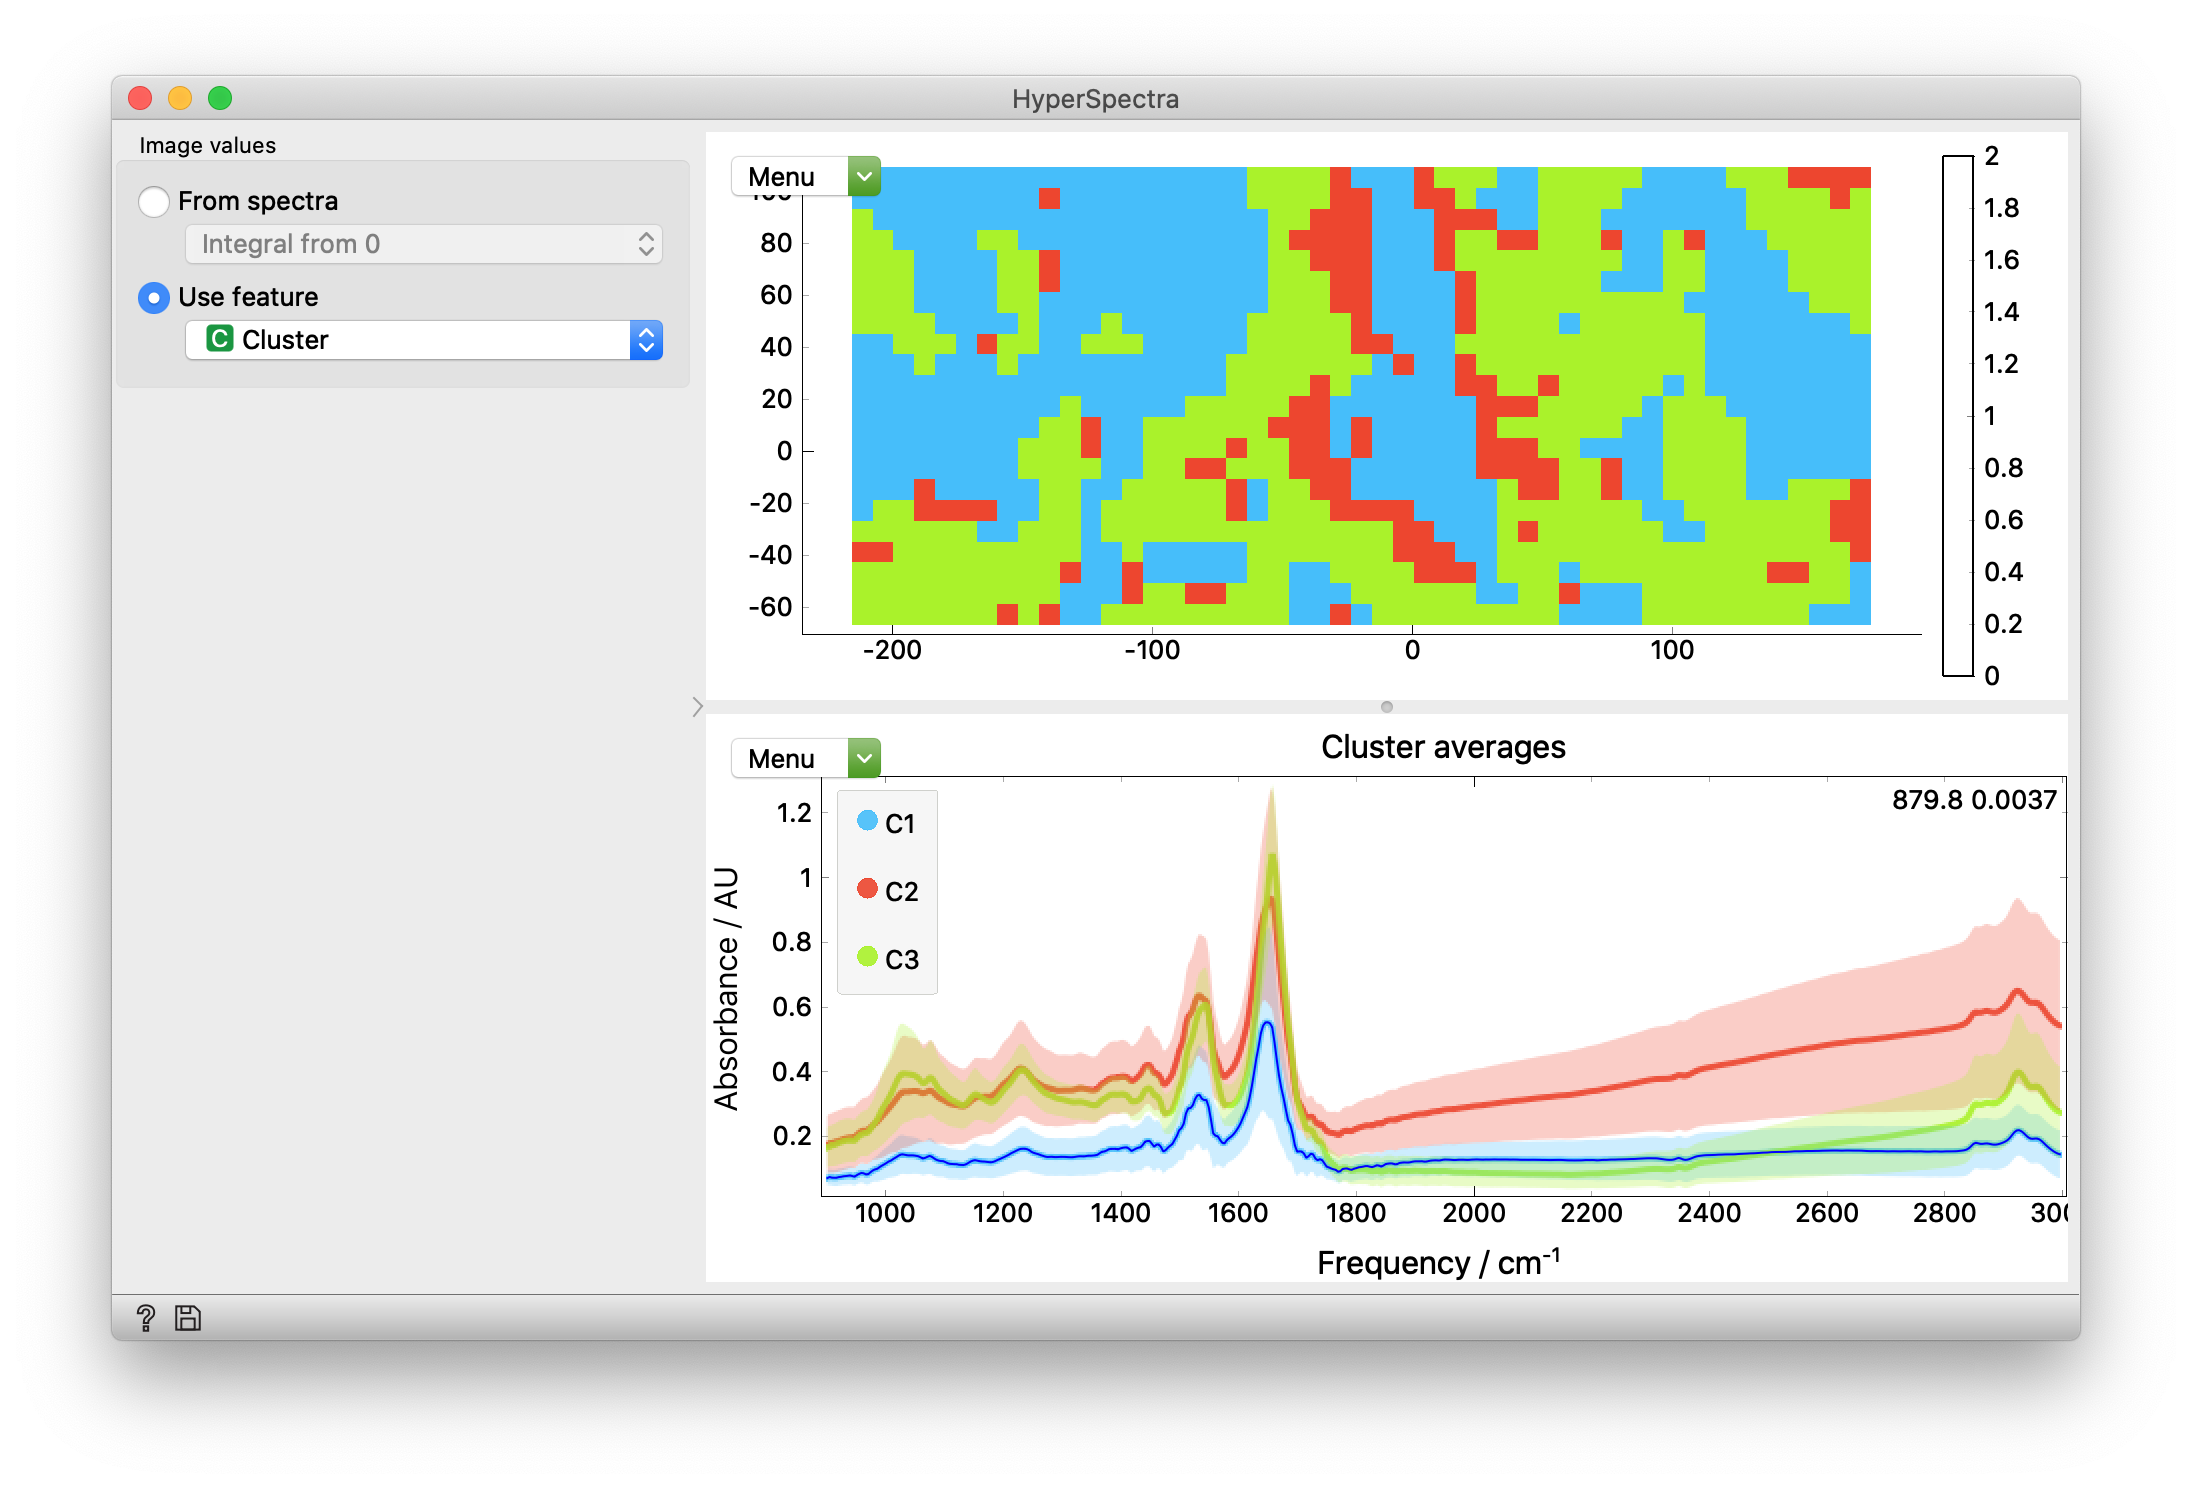
\includegraphics[scale=0.25]{graphics/ch-spectra_image_clustering/sp_image_clustering-fig2b.png}}
  \infinitewidthbox{\kmeans \hspace{-0.5cm} \hyperspectra}
  \vspace{-1.0cm}
  \caption{The \widget{Spectra} widget shows wrong predictions for the DNA class.}
  \label{ffig:spectra_image_clustering-fig2}
\end{figure*}

\vspace{0.8cm}

\begin{wrapfigure}{o}{1.1\textwidth}
  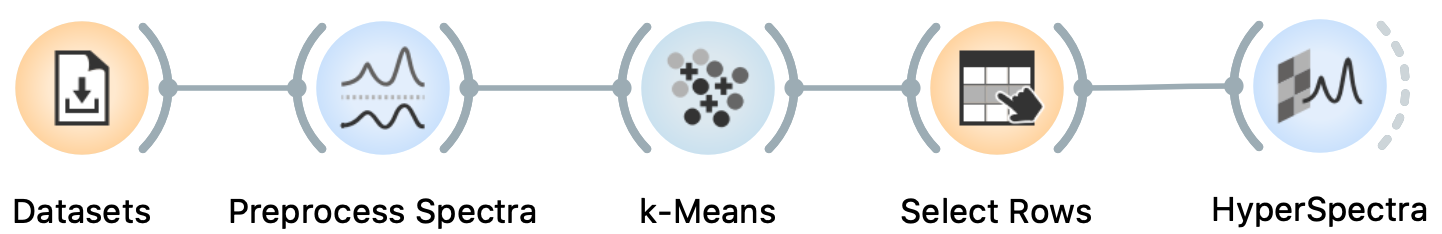
\includegraphics[scale=0.4]{graphics/ch-spectra_image_clustering/sp_image_clustering-fig3.png}%
  \label{fig:spectra_image_clustering-fig3}
\end{wrapfigure}

We see no meaningful clusters. Therefore, we need to preprocess the data. If we do it well, we see that a cluster corresponds to the background. We could remove it with the \widget{Select Rows} widget.

\begin{figure*}[h]
  \vspace{-0.3cm}
  \newcommand{\hyperspectra}{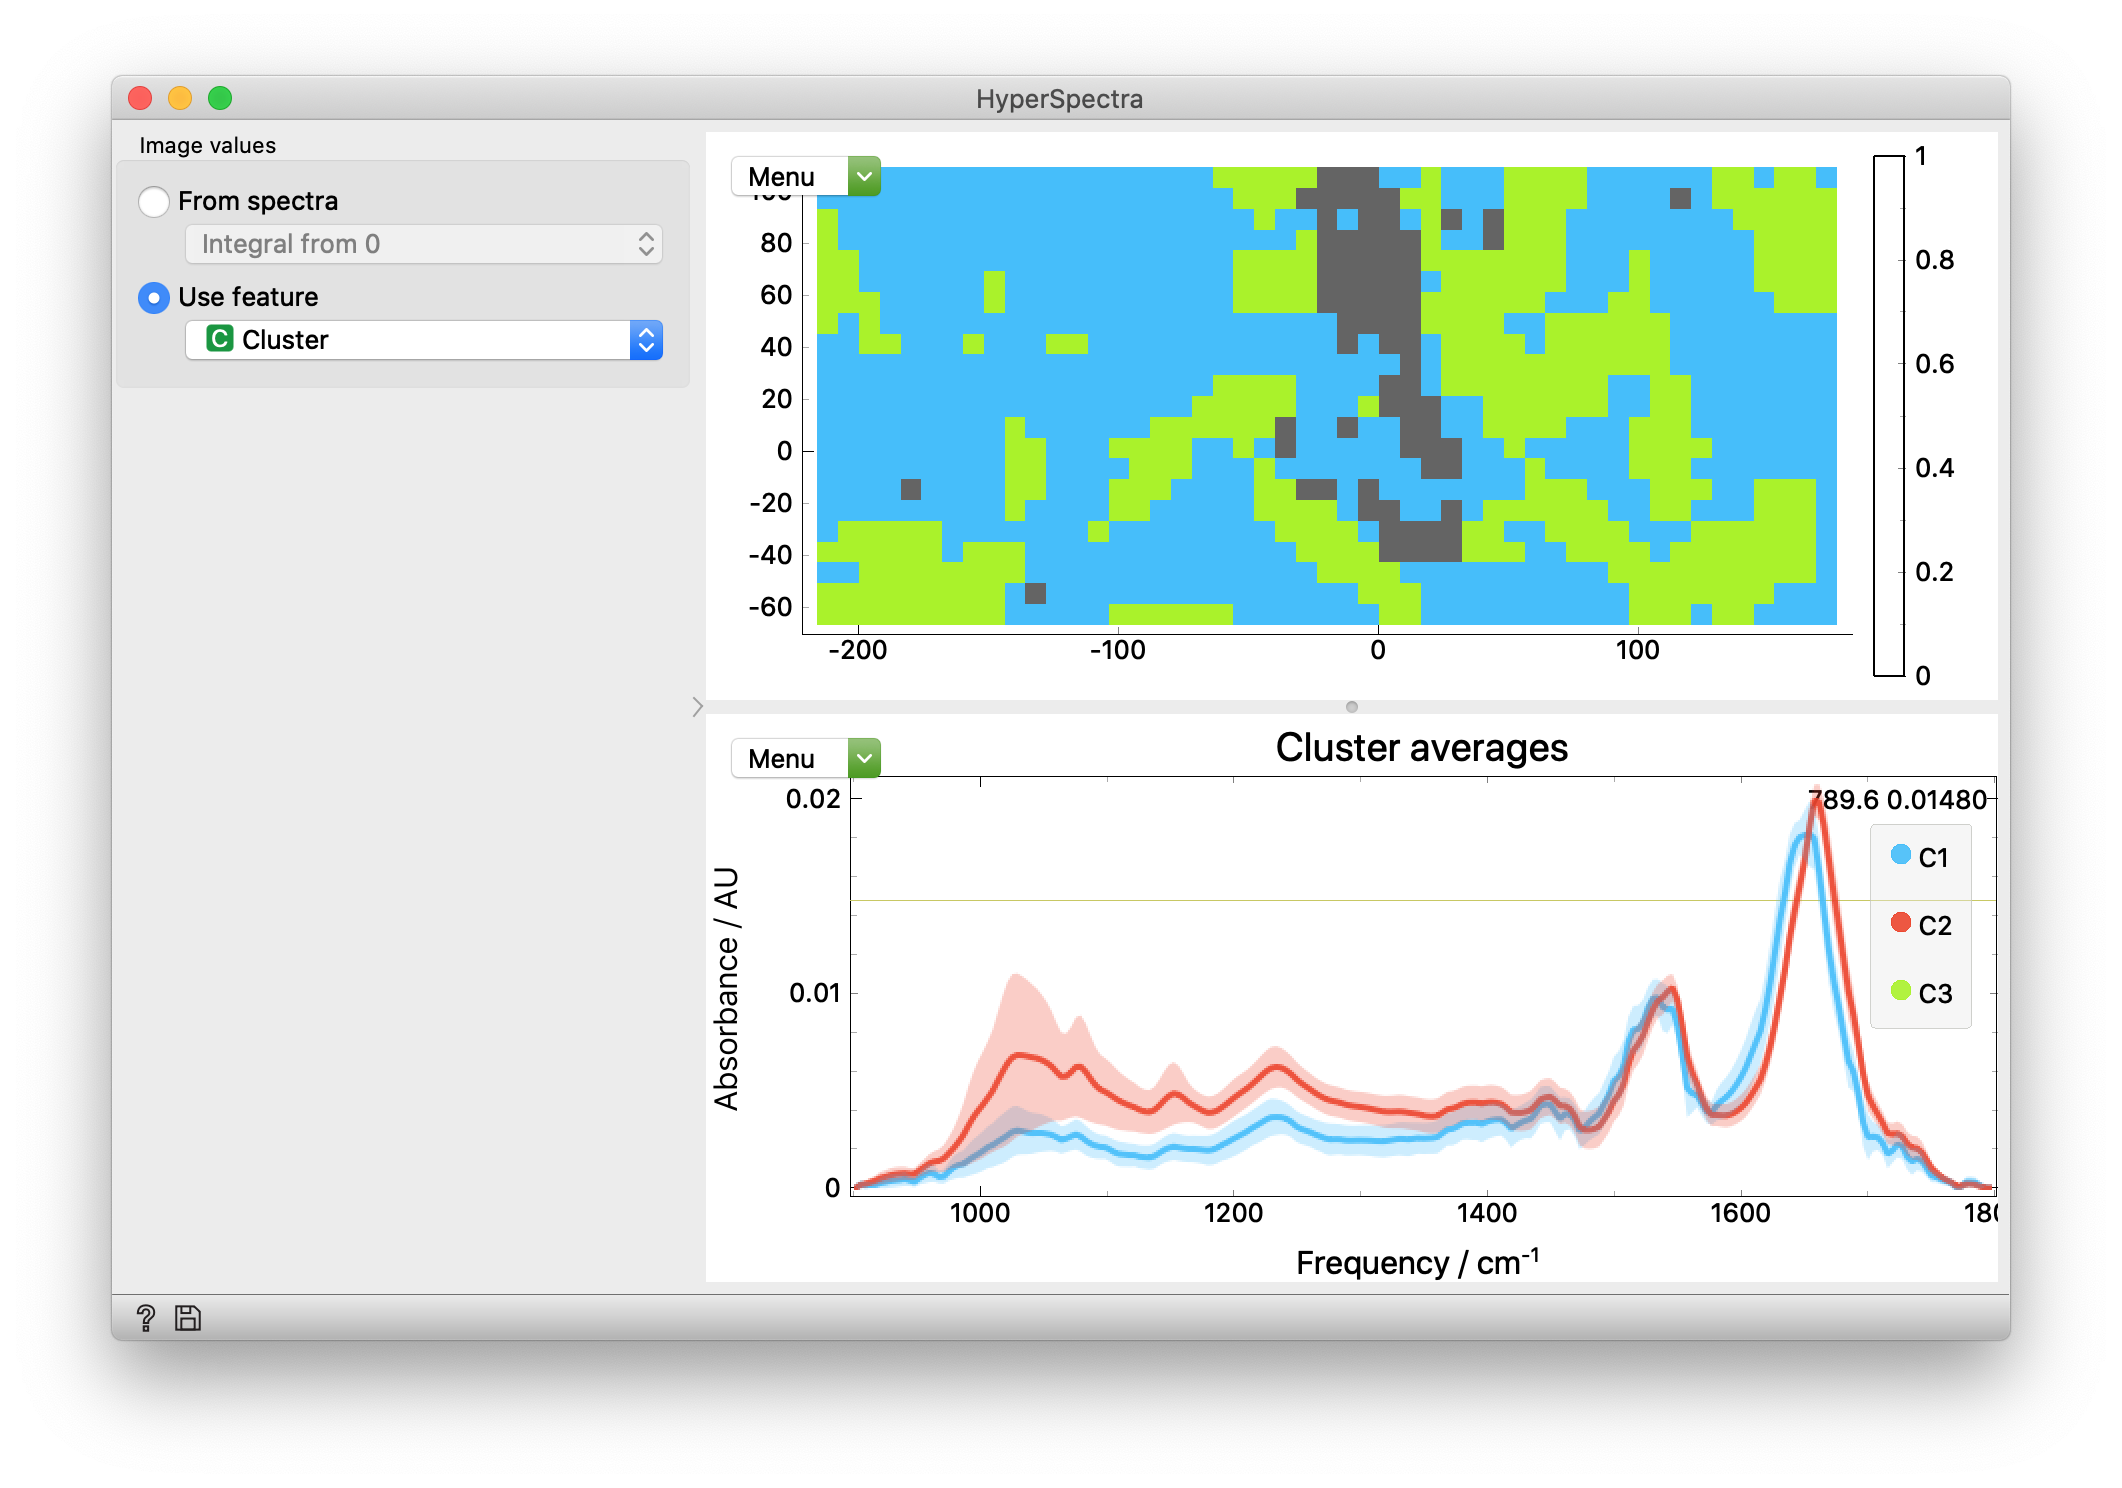
\includegraphics[scale=0.25]{graphics/ch-spectra_image_clustering/sp_image_clustering-fig4b.png}}
  \newcommand{\selectrows}{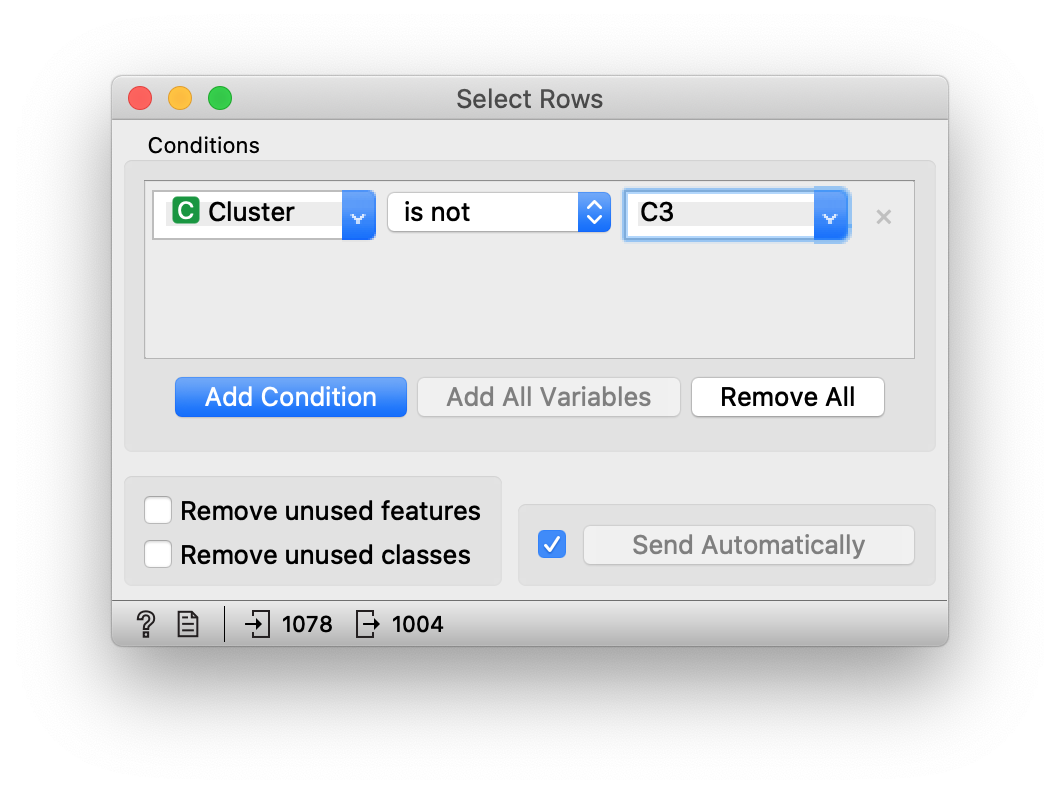
\includegraphics[scale=0.45]{graphics/ch-spectra_image_clustering/sp_image_clustering-fig4a.png}}
  \infinitewidthbox{\selectrows \hspace{-0.5cm} \hyperspectra}
  \vspace{-1.cm}
  \caption{The \widget{Spectra} widget shows wrong predictions for the DNA class.}
  \label{ffig:spectra_image_clustering-fig4}
\end{figure*}
